\clearpage
\subsection{Синтез алгоритмов управления}
\subsubsection{Вычисление угла коммутации}
Как было показано в разделе \ref{sec_feedback_control}, эффективность управления
повышается, если переключать фазы двигателя исходя c переменным углом коммутации
зависящем от скорости вращения ротора.

В общем случае согласно \ref{sec_feedback_control} исходными переменными во
времени параметрами для расчета угла коммутации являются текущая скорость и
требуемый момент.
Скорость важна из--за ненулевой индуктивности обмоток смотри
рис. (\ref{graph_speed_and_angle_comutation}).
В результате которой возникает постоянная задержка по времени нарастания тока в
обмотках двигателя, и следовательно задержка включения фазы.

Согласно уравнению (\ref{winding_current_with_pwm_control_1}) и
    (\ref{winding_current_with_pwm_control_0})
для нашего двигателя с параметрами:
Период ШИМ:
$$
    T_\textit{шим} = \frac{1024}{6 \cdot 10^7} = 1.706667 \cdot 10^{-5}, \text{с}
$$
Электрическая постоянная обмотки фазы для паралельного включения:
$$
    T = \frac{L}{R} = 2.14286 \cdot 10^{-3}, \text{c}
$$
$$
    \sigma = T / T_\textit{шим} = 125.55
$$
Для коэффициента заполнения:
$$
    \zeta = 0.15
$$
построим график измения тока в обмотках на протяжение первого импульса ШИМ в
импульсе управления с нулевым начальным током (рис. \ref{i_step__varepsilon}).

\begin{figure}
    \centering
    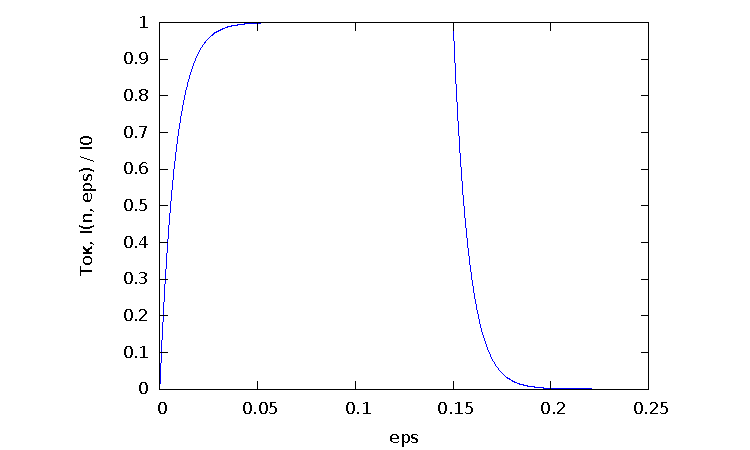
\includegraphics[width=\linewidth, keepaspectratio]
                    {./src/pictures/i_step__varepsilon.pdf}
    \caption{Форма тока в обмотках на протяжение 1--го импульса ШИМ}
    \label{i_step__varepsilon}
\end{figure}

Очевидно, что для наших параметров двигателя в заданном диапазоне скоростей
задержкой нарастания тока в коррекции угла коммутации можно пренабречь.

Вторым параметром системы задающим угол коммутации в системе является целевой
момент.
Угол коммутации задает форму кривой изменения момента на протяжении шага
рис. \ref{pic_moment_from_angle}.
Оптимальный угол коммутации с точки зрения максимизации момента без учета
поправки на задержку нарастания очевидно: $1.5 \theta_\text{шаг.}$.

\begin{figure}[h]
    \centering
    \begin{tikzpicture}[scale=2.5, samples = 1000]
        \def\xmin{-1.5}
        \def\xmax{3.5}
        \def\ymin{-1.5}
        \def\ymax{1.5}

        % axes
        \draw[thick, >=angle 45, ->] (\xmin,0) -- (\xmax,0)
            node[anchor=south west] {$\Delta \theta,$ рад.};
        \draw[thick, >=angle 45, ->] (0,\ymin) -- (0,\ymax+0.5)
            node[anchor=south west] {$\tau$};

        % xticks
        \foreach \x in {-1,1,2,3}
            \node at (\x, 0) [anchor=south west] {$\x\theta$};

        % x tick lines
        \foreach \x in {-1,0,1,2,3}
            \draw[thin, densely dotted] (\x,\ymin) -- (\x,\ymax);

        % yticks
        \foreach \y in {-1,1}
            \node at (0, \y) [anchor=south west] {\y};

        % y tick lines
        \foreach \y in {-1,1}
            \draw[thin, densely dotted] (\xmin,\y) -- (\xmax,\y);

        % curve
        \draw plot[smooth, domain = \xmin:\xmax, thick] (\x,{sin(\x*1.57 r)});

        % commutation angle
        \def\comm{1.3}
        \def\commMinusStep{0.3}
        \draw[thin, dashed] (\comm,\ymin) -- (\comm,\ymax+0.5);
        \draw[thin, dashed] (\commMinusStep,\ymin) -- (\commMinusStep,\ymax+0.5);

        \draw[<->, >=angle 45, thin] (0,\ymax-0.1) -- (\commMinusStep,\ymax-0.1);
        \draw[thin] (-1,\ymax-0.1) -- (0,\ymax-0.1);
        \node at (0, \ymax-0.1) [anchor=south east] {$\theta_\text{ком} - \theta_\text{шаг}$};

        \draw[<->, >=angle 45, thin] (0,\ymax+0.3) -- (\comm,\ymax+0.3);
        \draw[thin] (-0.4,\ymax+0.3) -- (0,\ymax+0.3);
        \node at (0, \ymax+0.3) [anchor=south east] {$\theta_\text{ком}$};

    \end{tikzpicture}
    \caption{Зависимость момента от угла рассогласования}
    \label{pic_moment_from_angle}
\end{figure}

Осюда несложная зависимость для угла коммутации от целевого момента следующая из
формулы \ref{torque_from_rotor_deviation}
и \ref{eq_average_moment_to_rotor_on_control_pulse}:

$$
    \tau_\textit{двиг} =
        \tau_{\textit{шаг}} =
            K_{M} I_{M} N_{r} ( \theta_{\textit{ком}}
                                - \frac{ \theta_{\textit{шаг}} }{ 2 }
            )
$$

Полный момент отрабатываемый двигателем:
\begin{equation}
    \label{eq_motor_torque}
    \tau_\textit{двиг} =
        \tau_\textit{цель}
        + \tau_\textit{стат}
        + \tau_\textit{вязк}
\end{equation}

\begin{equation}
    \label{eq_commutation_angle}
    \theta_{\textit{ком}} =
    \frac{ \tau_\textit{цель} + \tau_\textit{стат} + \tau_\textit{вязк} }
         { K_{M} \cdot I_{M} \cdot N_{r} }
    + \frac{ \theta_{\textit{шаг}} }{ 2 }
\end{equation}

При этом важно ограничить угол коммутации сверху и снизу, так как расчетное
значение может значительно выходить за допустимый диапазон описаный в разделе
\ref{sec_feedback_control}
$$
    0 < \theta_{\textit{ком}} \leq 2
$$

\clearpage
\subsubsection{ОС по положению}
\label{fedback_control_algo}
Здесь и далее будем рассматривать принципы переключения активной фазы шагового
двигателя на примере простого четырёхфазного шагового двигателя.
Условно, процесс движения ротора шагового двигателя можно разделить на 3
элементарные части (<<зоны>>), которые соответствую трём действиям системы
упраления в процессе движения:

\begin{enumerate}
    \item Зона движения
    \item Зона переключения
    \item Зона выпада из сихронизма
\end{enumerate}

Каждой зоне соответсвует свое условие на величину рассогласования векторов
магнитного поля.

Таким образом, решение о необходимости переключения фаз принимается на основании
анализа того, в какой зоне находится ротор двигателя в данный момент. Найдём
условия, необходимые для этого, проанализировав процесс вращения ротора
двигателя в положительном и отрицательном направлениях.

\textit{Зоной движения} будем называть зону, в которой ротор совершает движения
в рамках текущего шага, включена нужная фаза и, следовательно, перелюкчение не
требуется.

\textit{Зоной переключения} будем называть зону, в которой пришло время
включения следующей фазы. Зафиксировав, что ротор находится в этой зоне, модуль
ОС по положению даёт команду шаговому модулю сделать один шаг в направлении
движения.

\textit{Зоной выпада из синхронизма} будем называть зону, в которую попадает
ротор двигателя в случае пропуска шагов или возникновения некоторой
непредвиденной ситуации (например, удара, отбросившего ротор назад).
Так как зоны не пересекаются, но граничат друг с другом, зону выпада из
синхронизма можно определить как всю область вне зон движения и переключения.

В соответствие с принятыми обозначениями, будем обозначать угловое положение
ротора (угловое положение вектора магнитного поля ротора) как $\theta$.
Угловое положение вектора магнитного поля статора обозначим $\phi_\textit{акт}$.

\paragraph{Зоны движения и переключения}
\subparagraph{Движение в положительном направлении}
\begin{figure}
    \centering
    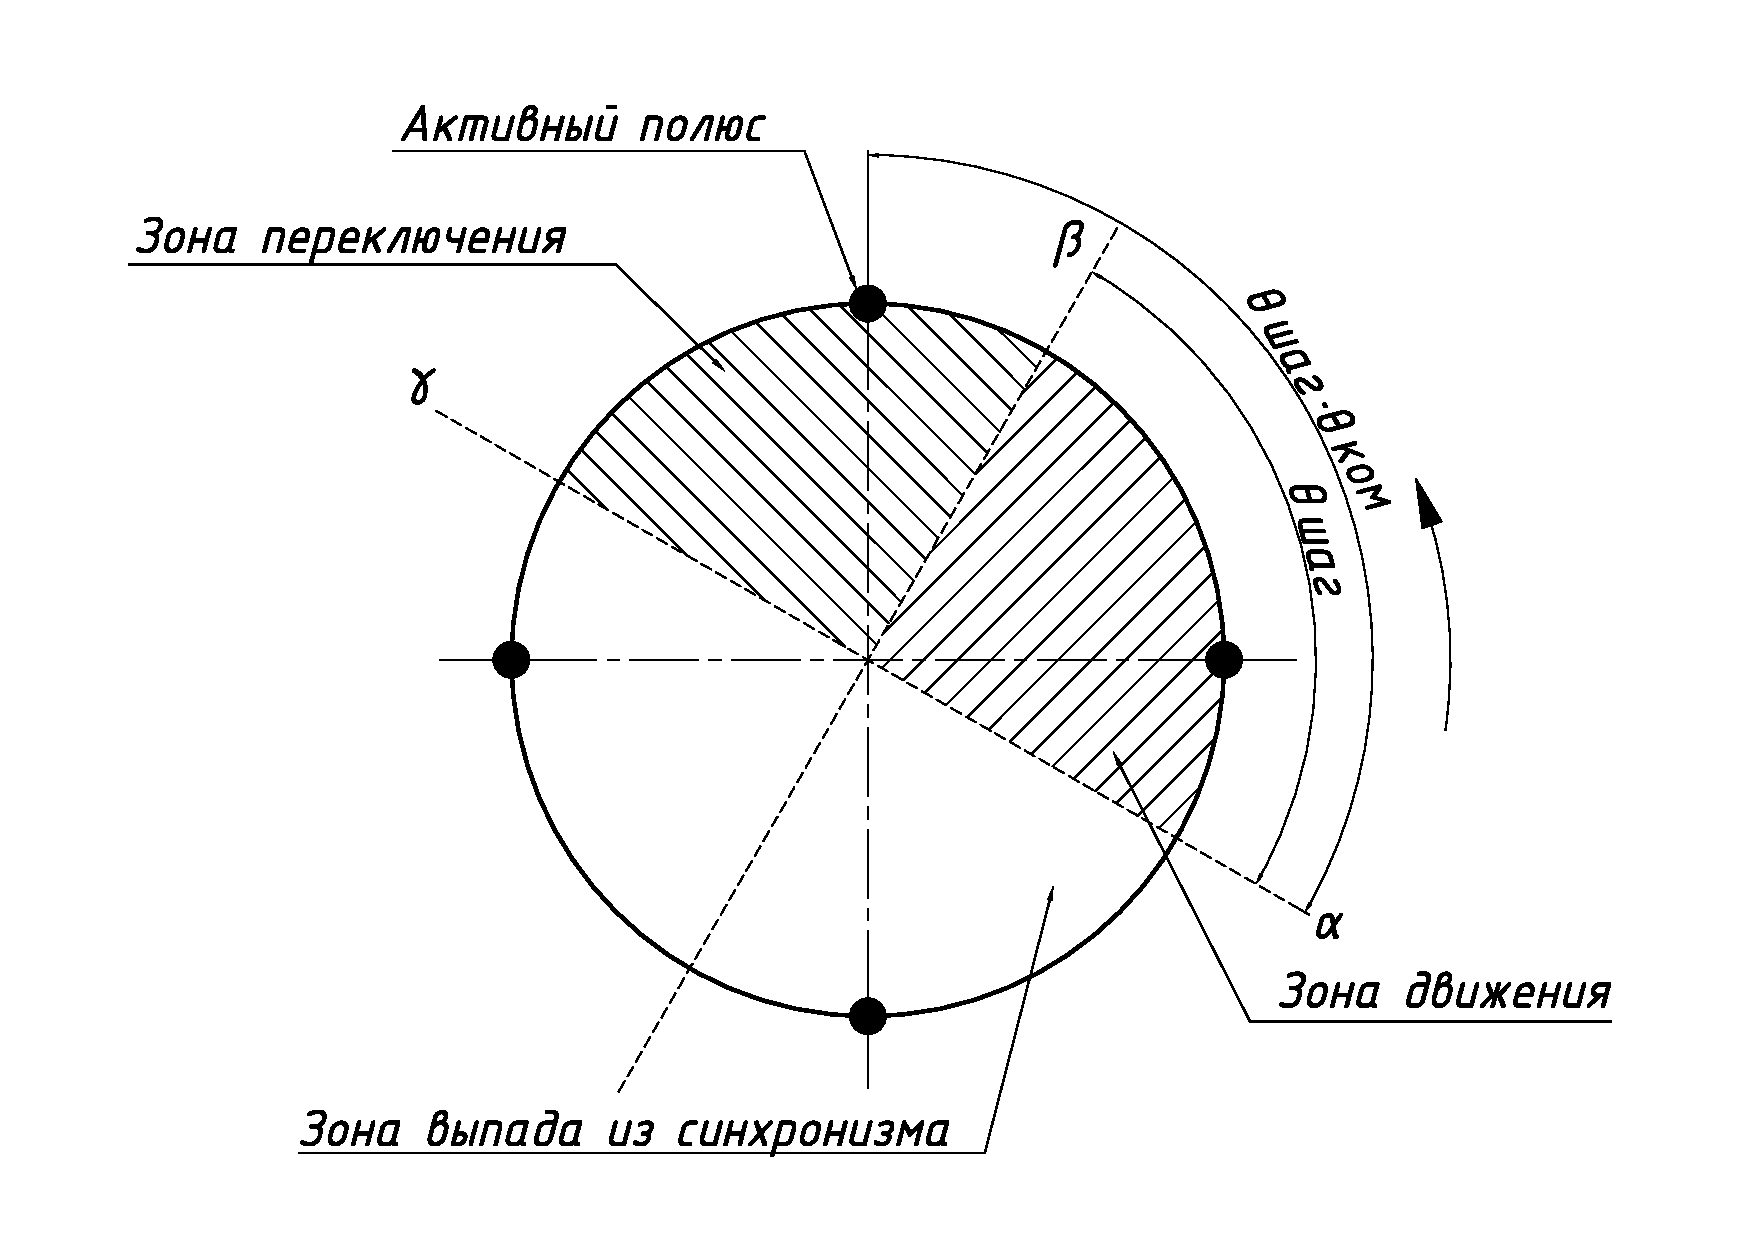
\includegraphics[width=0.7\textwidth, keepaspectratio]
                    {./src/pictures/feedback_control/pole_switch_zones_with_positive_dir}
    \caption{Зоны рассогласований магнитных векторов ротора и статора при вращении в положительном направлении}
    \label{pole_switch_zones_with_positive_dir}
\end{figure}

В зоне движения угловое положение ротора $\theta$ будет удовлетворять следующему
условию:
$$
    \alpha \leq \theta < \beta
$$

\begin{equation}
    \label{movement_zone_posit_dir_for_curr_pos}
    \phi_\textit{акт} - \theta_\textit{ком}
    \leq \theta <
    \phi_\textit{акт} - (\theta_\textit{ком} - \theta_\textit{шаг})
\end{equation}

Преобразовав это неравенство, получим выражение, описывающее границы зоны движения
в величинах рассогласования векторов магнитных полей статора и ротора:

\begin{equation}
    \label{movement_zone_posit_dir_for_delta}
    \theta_\textit{ком} - \theta_\textit{шаг}
    < \phi_\textit{акт} - \theta
    \leq \theta_\textit{ком}
\end{equation}

В зоне переключения угловое положение ротора $\theta$ будет удовлетворять следующему условию:
$$
    \beta \leq \theta < \gamma
$$

\begin{equation}
    \label{switch_zone_posit_dir_for_curr_pos}
    \phi_\textit{акт} - (\theta_\textit{ком} - \theta_\textit{шаг})
    \leq \theta <
    \phi_\textit{акт} - (\theta_\textit{ком} - 2\theta_\textit{шаг})
\end{equation}

Преобразовав это неравенство, получим выражение, описывающее границы зоны переключения
в величинах рассогласования векторов магнитных полей статора и ротора:

\begin{equation}
    \label{switch_zone_posit_dir_for_delta}
    \theta_\textit{ком} - 2\theta_\textit{шаг}
    < \phi_\textit{акт} - \theta
    \leq \theta_\textit{ком} - \theta_\textit{шаг}
\end{equation}


\subparagraph{Движение в отрицательном направлении}
\begin{figure}
    \centering
    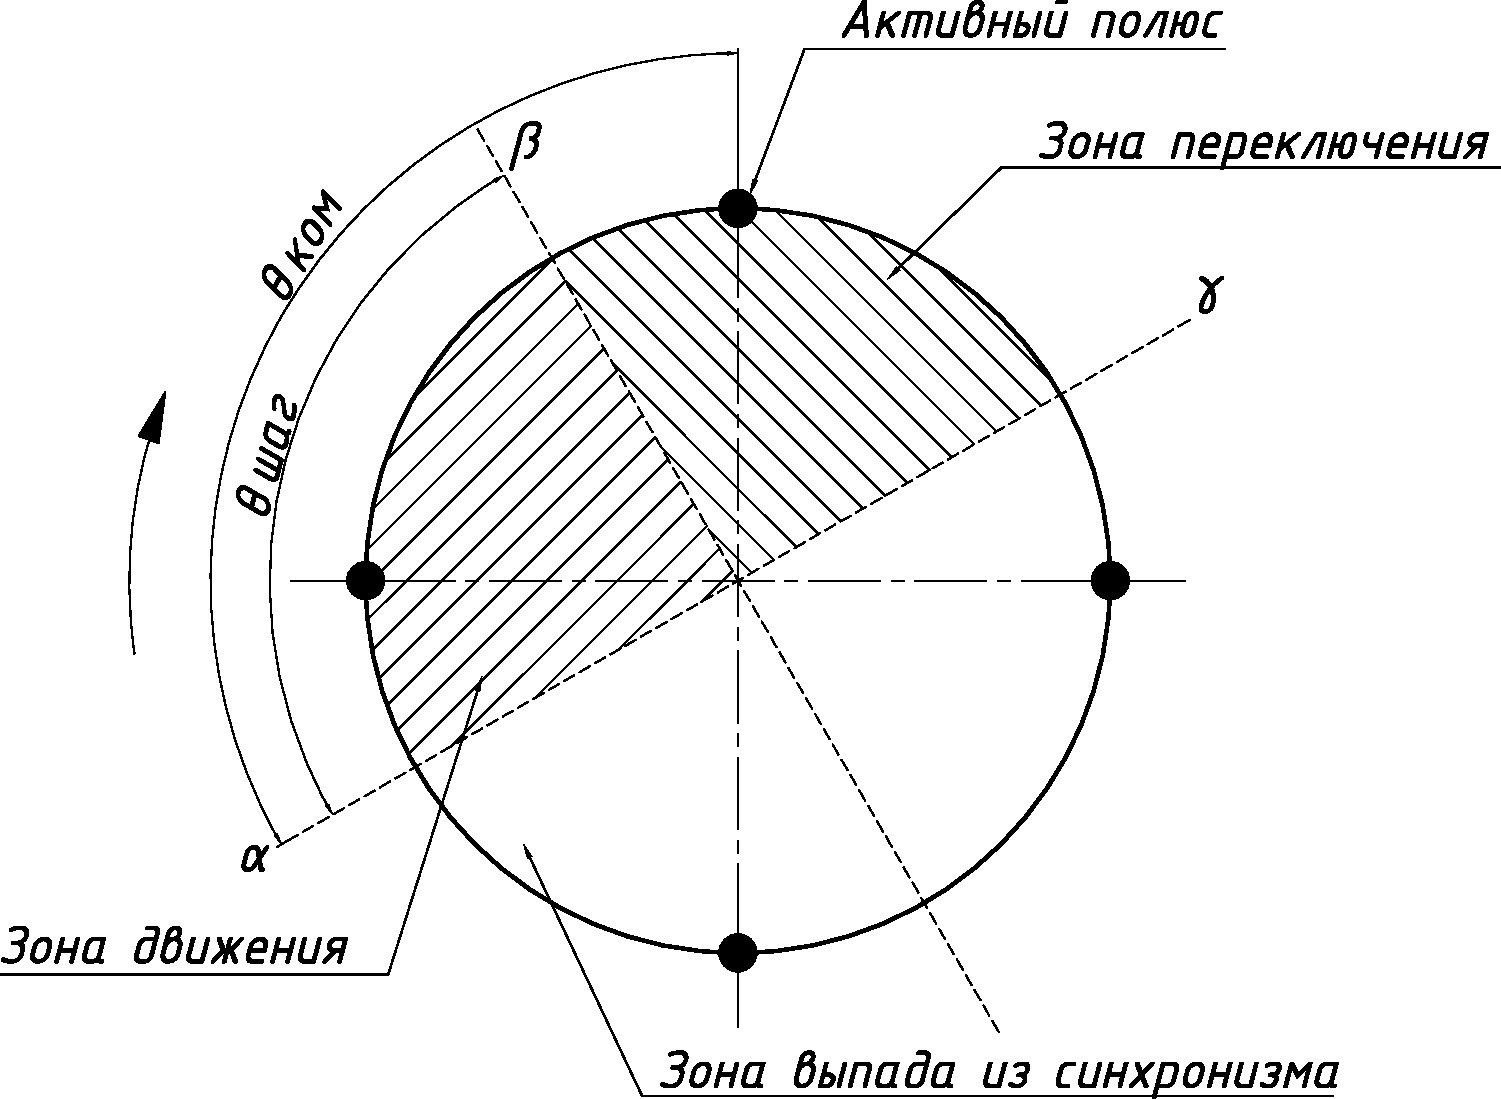
\includegraphics[width=0.7\textwidth, keepaspectratio]
                    {./src/pictures/feedback_control/pole_switch_zones_with_negative_dir}
    \caption{Зоны рассогласований магнитных векторов ротора и статора при вращении в отрицательном направлении}
    \label{pole_switch_zones_with_negative_dir}
\end{figure}

В зоне движения угловое положение ротора $\theta$ будет удовлетворять следующему условию:
$$
    \beta < \theta \leq \alpha
$$

\begin{equation}
    \label{movement_zone_negat_dir_for_curr_pos}
    \phi_\textit{акт} + \theta_\textit{ком} - \theta_\textit{шаг}
    <     \theta
    \leq \phi_\textit{акт} + \theta_\textit{ком}
\end{equation}

Преобразовав это неравенство, получим выражение, описывающее границы зоны
движения в величинах рассогласования векторов магнитных полей статора и ротора:

\begin{equation}
    \label{movement_zone_negat_dir_for_delta}
    -\theta_\textit{ком}
    \leq \phi_\textit{акт} - \theta
    < \theta_\textit{шаг} - \theta_\textit{ком}
\end{equation}

В зоне переключения угловое положение ротора $\theta$ будет удовлетворять
следующему условию:
$$
    \gamma < \theta \leq \beta
$$

\begin{equation}
    \label{switch_zone_negat_dir_for_curr_pos}
    \phi_\textit{акт} + \theta_\textit{ком} - 2\theta_\textit{шаг}
    < \theta \leq
    \phi_\textit{акт} + \theta_\textit{ком} - \theta_\textit{шаг}
\end{equation}

Преобразовав это неравенство, получим выражение, описывающее границы зоны
переключения в величинах рассогласования векторов магнитных полей статора и
ротора:

\begin{equation}
    \label{switch_zone_negat_dir_for_delta}
    \theta_\textit{шаг} - \theta_\textit{ком}
    \leq \phi_\textit{акт} - \theta
    < 2\theta_\textit{шаг} - \theta_\textit{ком}
\end{equation}

\subsubsection{Синхронное управление}
C помощью формулы (\ref{eq_synchronized_control_max_frequency}) для линейного
ускорения двигателя и формулы (\ref{eq_synchronized_control_min_frequency}) для
линейного торможения двигателя получим предельные частоты для тактирования
переключения обмоток в управлении без обратоной связи. Здесь и далее будем
именовать такое управление синхронным.

Для синхронного управления из формулы
(\ref{eq_average_moment_to_rotor_on_control_pulse}) получим соответсвие момнта току в обмотках
двигателя. Формула (\ref{eq_average_moment_to_rotor_on_control_pulse}) была
выведена для управления по датчику, но она будет справедлива и для синхронного
управления, если принять угол коммутации равным 1:
$\theta_\textit{ком} = \theta_\textit{шаг}$.
